\documentclass[]{comunicaciones}
\labelpaper[year =2014 , month =12, volume =7, number =2 , firstpage =115 ]
%Cargar los paquetes necesarios aqu?
\usepackage{enumitem}  % format a list as to remove the spaces between list items
\usepackage[usenames,dvipsnames,svgnames,table]{xcolor} % para usar colores

% New for newcommand, proglang and code
\newcommand{\pkg}[1]{{\normalfont\fontseries{b}\selectfont #1}}
\let\proglang=\textsf
\let\code=\texttt

\begin{document}
\title[maintitle = Aplicaciones \pkg{shiny} para apoyar los procesos de aprendizaje de pruebas de hip?tesis (t?tulo tentativo a mejorar),
       secondtitle = T?tulo en ingl?s
       shorttitle = T?tulo corto]       

\begin{authors}
\author[firstname = Freddy,
surname = Hern?ndez Barajas,
%numberinstitution = 1,
affiliation = {Profesor asistente, Universidad Nacional de Colombia, Sede Medell\'in.},
email = fhernanb@unal.edu.co]
\author[firstname = Olga Cecilia,
surname = Usuga Manco,
%numberinstitution = 2,
affiliation = {Profesora asociada, Universidad de Antioquia, Medell\'in.},
email = olga.usuga@udea.edu.co]
\author[firstname = Santiago Humberto,
surname = Londo?o Restrepo,
%numberinstitution = 2,
affiliation = {Profesor de Planta, Corporaci\'on Universitaria Americana.},
email = slondono@coruniamericana.edu.co]
\end{authors}

\begin{mainabstract}
Resumen del art?culo.
\textcolor{red}{A cargo de Olga y Freddy.}
\keywords{Palabras claves}
\end{mainabstract}

\begin{secondaryabstract}
Resumen en ingl?s.
\textcolor{red}{A cargo de Olga y Freddy.}
\keywords{Palabras claves en ingl?s}
\end{secondaryabstract}

%%%%%%%%%%%%%%%%%%%%%%%%%%%%%%%%%%%%%%%%%%%%%%%%%%%%%%%%%%%%%%%%%%%%%%%%%%%%%%%%%%%%%%%%%%%%%%%%%%%%
\section{Introducci?n}
\textcolor{red}{A cargo de Olga.}


%%%%%%%%%%%%%%%%%%%%%%%%%%%%%%%%%%%%%%%%%%%%%%%%%%%%%%%%%%%%%%%%%%%%%%%%%%%%%%%%%%%%%%%%%%%%%%%%%%%%
\section{Pruebas de hip?tesis}
Bla bla bla.

%%%%%%%%%%%%%%%%%%%%%%%%%
\subsection{Prueba de hip?tesis para la varianza}
Suponga que se tiene una muestra aleatoria $x_1, x_2, \ldots, x_n$ proveniente de una poblaci?n normal. Se desea estudiar la hip?tesis nula $H_0: \sigma^2 = \sigma_0^2$ y se sospecha que la varianza $\sigma^2$ podr?a estar en alguna de las siguientes situaciones (hip?tesis alterna):
\begin{enumerate}[noitemsep, nolistsep]
	\item $H_1: \sigma^2 < \sigma_0^2$
	\item $H_1: \sigma^2 \neq \sigma_0^2$
	\item $H_1: \sigma^2 > \sigma_0^2$
\end{enumerate}
El estad?stico para realizar la prueba es:
$$\chi_0^2=\frac{(n-1) s^2}{\sigma_0^2},$$
donde $s$ desviaci?n est?ndar muestral. Bajo la suposici?n de que $H_0$ es verdadera, $\chi_0^2$ tiene distribuci?n $\chi^2$ con $n-1$ grados de libertad \cite{Montgomery03}.

%%%%%%%%%%%%%%%%%%%%%%%%%
\subsection{Prueba de hip?tesis para la media}
Suponga que se tiene una muestra aleatoria $x_1, x_2, \ldots, x_n$ proveniente de una poblaci?n normal. Se quiere estudiar la hip?tesis nula $H_0: \mu = \mu_0$ y se sospecha que la media $\mu$ podr?a estar en alguna de las siguientes situaciones (hip?tesis alterna):
\begin{enumerate}[noitemsep, nolistsep]
	 \item $H_1: \mu < \mu_0$
	 \item $H_1: \mu \neq \mu_0$
	 \item $H_1: \mu > \mu_0$
\end{enumerate}
El estad?stico para realizar la prueba es:
$$t_0=\frac{\bar{x} - \mu_0}{s/\sqrt{n}},$$
donde $\bar{x}$ y $s$ son la media y desviaci?n est?ndar muestrales respectivamente. Bajo la suposici?n de que $H_0$ es verdadera, el estad?stico $t_0$ tiene distribuci?n $t$-student con $n-1$ grados de libertad \cite{Walpole12}.

Si se d? el caso en que la muestra aleatoria no proviene de una poblaci?n normal pero se cumple que $n \geq 40$, entonces en virtud del Teorema del L?mite Central, el estad?stico para realizar la prueba es:
$$z_0=\frac{\bar{x} - \mu_0}{s/\sqrt{n}},$$
y en esta situaci?n el estad?stico $z_0$ tiene una distribuci?n $N(0, 1)$. 

En cualquiera de los casos, la hip?tesis nula $H_0$ se rechaza si el valor-P es menor que el nivel de significancia fijado previamente por el analista.

%%%%%%%%%%%%%%%%%%%%%%%%%
\subsection{Prueba de hip?tesis para la proporcion}
\textcolor{red}{A cargo de Olga.}

%%%%%%%%%%%%%%%%%%%%%%%%%
\subsection{Prueba de hip?tesis para el cociente de varianzas}\label{phvars}
Suponga que se tienen dos muestras aleatorias que provienen de poblaciones normales as?:
\begin{itemize}[noitemsep, nolistsep]
	\item $n_1$ observaciones $x_{11}, x_{12}, \ldots, x_{1,n1}$ de una poblaci?n I con  varianza $\sigma^2_1$, 
	\item $n_2$ observaciones $x_{21}, x_{22}, \ldots, x_{2,n2}$ de una poblaci?n II con varianza $\sigma^2_2$,
	\item ambas muestras son independientes entre s?.
\end{itemize}
Se quiere estudiar la hip?tesis nula $H_0: \sigma_1^2 / \sigma_2^2 = 1$ y se sospecha que el cociente de varianzas $\sigma_1^2 / \sigma_2^2$ podr?a estar en alguna de las siguientes situaciones (hip?tesis alterna):
\begin{enumerate}[noitemsep, nolistsep]
	\item $H_1: \sigma_1^2 / \sigma_2^2 < 1$
	\item $H_1: \sigma_1^2 / \sigma_2^2 \neq 1$
	\item $H_1: \sigma_1^2 / \sigma_2^2 > 1$
\end{enumerate}
El estad?stico para realizar la prueba es:
$$f_0=\frac{s_1^2}{s_1^2},$$

donde $s_1^2$ y $s_2^2$ son las varianzas muestrales de las poblaciones I y II respectivamente. El estad?stico $f_0$, bajo la suposici?n de que $H_0$ es verdadera, tiene distribuci?n $f$ con $n_1-1$ grados de libertad en el numerador y $n_2-1$ grados de libertad en el denominador \cite{Devore16}.

En esta prueba, al no rechazar la hip?tesis nula $H_0$, se concluye que $\sigma_1^2 / \sigma_2^2 = 1$ lo que implica en t?rminos pr?cticos que $\sigma_1^2 = \sigma_2^2$, es decir que las varianzas poblacionales se pueden considerar iguales.

%%%%%%%%%%%%%%%%%%%%%%%%%
\subsection{Prueba de hip?tesis para la diferencia de medias}
Suponga que se tienen dos muestras aleatorias que provienen de poblaciones normales as?:
\begin{itemize}[noitemsep, nolistsep]
	\item $n_1$ observaciones $x_{11}, x_{12}, \ldots, x_{1,n1}$ de una poblaci?n I con media $\mu_1$ y varianza $\sigma^2_1$,
	\item $n_2$ observaciones $x_{21}, x_{22}, \ldots, x_{2,n2}$ de una poblaci?n II con media $\mu_2$ y varianza $\sigma^2_2$,
	\item ambas muestras son independientes entre s?.
\end{itemize}
Se quiere estudiar la hip?tesis nula $H_0: \mu_1 - \mu_2 = \delta_0$ y se sospecha que la diferencia de medias $\mu_1 - \mu_2$ podr?a estar en alguna de las siguientes situaciones (hip?tesis alterna):
\begin{enumerate}[noitemsep, nolistsep]
	\item $H_1: \mu_1 - \mu_2 < \delta_0$
	\item $H_1: \mu_1 - \mu_2 \neq \delta_0$
	\item $H_1: \mu_1 - \mu_2 > \delta_0$
\end{enumerate}
Para realizar esta prueba de hip?tesis se deben diferenciar dos casos, uno en el que las varianzas son iguales y otro caso en el que las varianzas son diferentes, esto se puede chequear utilizando la prueba descrita en la secci?n \ref{phvars} del presente art?culo. Para cada uno de los casos descritos hay un estad?stico de prueba y una distribuci?n del estad?stico, a continuaci?n se presentan los dos casos en detalle.
\subsubsection{Caso 1: varianzas poblacionales iguales $\sigma_1^2 = \sigma_2^2$}
En este caso el estad?stico para realizar la prueba es:
$$t_0=\frac{\bar{x}_1 - \bar{x}_2 - \delta_0}{S_p \sqrt{\frac{1}{n_1} + \frac{1}{n_2}}},$$
donde $\bar{x}_1$ y $\bar{x}_2$ son las medias muestrales de las poblaciones I y II respectivamente, la cantidad $S_p^2$ es una varianza combinada y se calcula como:
$$S_p^2=\frac{(n_1-1)s_1^2+(n_2-1)s_2^2}{n_1+n_2-2},$$
donde $s_1^2$ y $s_2^2$ son las varianzas muestrales de las poblaciones I y II respectivamente.

En este caso el estad?stico $t_0$, bajo la suposici?n de que $H_0$ es verdadera, tiene distribuci?n $t$-student con $n_1+n_2-2$ grados de libertad \cite{Walpole12}.

\subsubsection{Caso 2: varianzas poblacionales diferentes $\sigma_1^2 \neq \sigma_2^2$}
En este caso el estad?stico para realizar la prueba es 
$$t_0=\frac{\bar{x}_1 - \bar{x}_2 - \delta_0}{\sqrt{\frac{s_1^2}{n_1} + \frac{s_2^2}{n_2}}}$$
En este caso el estad?stico $t_0$, bajo la suposici?n de que $H_0$ es verdadera, tiene distribuci?n $t$-student con $v$ grados de libertad \cite{Walpole12}, en donde $v$ se calcula como:
$$v=\frac{ \left( \frac{s_1^2}{n_1} + \frac{s_2^2}{n_2} \right)^2 }{ \frac{(s_1^2/n_1)^2}{n_1-1} + \frac{(s_2^2/n_2)^2}{n_2-1}}$$

%%%%%%%%%%%%%%%%%%%%%%%%%
\subsection{Prueba de hip?tesis para la diferencia de proporciones}
\textcolor{orange}{A cargo de Olga.}

%%%%%%%%%%%%%%%%%%%%%%%%%%%%%%%%%%%%%%%%%%%%%%%%%%%%%%%%%%%%%%%%%%%%%%%%%%%%%%%%%%%%%%%%%%%%%%%%%%%%
\section{Paquete \pkg{shiny}}
\textcolor{red}{A cargo de Santiago.}

Shiny es un paquete del software de código abierto conocido como R. Hace que sea posible crear facilmente aplicaciones o aplicativos web interactivos sin requerir conocimientos de HTML, CSS o JavaScript, solo se necesita saber R. Creado por \cite{Winston17} y mejorado con la ayuda de múltiples colaboradores como Mark Otto, Scott Jehl entre otros. Para mayor información visitar https://cran.r-project.org/web/packages/shiny/index.html

Un aplicativo web interactivo hoy en día es algo más común de lo imaginado, especialmente para aquellos que usan internet como su herramienta aliada en el trabajo, estudio o comunicación. Es muy probable que usted use almenos uno al día sin que se de cuenta de que eso, que le facilita la vida, es un aplicativo web. Por ejemplo los correos electrónicos, wikipedia, las tiendas online, los blogs, youtube y facebook son algunos de ellos, ¿los ha usado? Lo más seguro es que sí.

Ellos comparten tres características en común. La primera, se utilizan por medio de internet, cualquier persona con conexión puede hacer uso de ellos, algunos no son gratuitos así que no es suficiente con tener internet. Segunda, el usuario se encarga de administrar la entrada (input), es decir el usuario es quien decide que hacer con el aplicativo, por ejemplo si usted desea observar videos en youtube sobre su cantante favorito usted es quien digita sobre el cajón de texto (cajón de búsqueda) el nombre del cantante. Tercera, el aplicativo se encarga de la salida (outputs), es decir el aplicativo ejecuta de forma automática la entrada (input) suministrada por el usuario inicialmente y arroja un resultado que coincida con dicha entrada. Siguiendo nuestro ejemplo de youtube, al usted ingresar el nombre del cantante y luego de dar clic sobre el botón de buscar (botón con lupa) o luego de oprimir el botón enter, youtube (el aplicativo) se encarga de buscar automáticamente, todos los videos asociados al cantante. Adicionalmente muestra de forma ordenada en la pantalla de su computadora o télefono móvil la gran cantidad de videos que se puedan presentar. Notar que el aplicativo hace el trabajo duro: buscar miles de videos entre millones que coincidan con los deseos del usuario y mostrarlos de forma agradable, Wow un milagro.

Shiny permite al desarrollador de aplicativos web interactivos integrar esas tres características sin mayor esfuerzo. Shiny proporciona una gran variedad de formas en cómo el usuario puede administrar las entradas y proporciona diversar maneras de expresar las salidas sin necesidad de que el desarrollador tenga conocimiento del código fuente que crea dichas entradas y salidas. Sólo se debe preocupar por aspectos como la forma del aplicativo y sobre cómo debe reaccionar automáticamente la salida (output) ante los valores proporcionados en la entrada (input). Ahora, sí la preocupacón es cómo almacenar en la web o en internet el apliactivo creado, no hay de qué preocuparse, pues shiny proporciona diversas formas de alojamiento en servidores. De esta manera, es posible crear aplicaciones hermosas, receptivas y potentes con sólo tener conocimiento del lenguaje R.

Un aplicativo web creado a través del paquete shiny esta conformado por dos archivos: archivo ui.R y archivo server.R. En el archivo ui.R se escribe el código que se encargará de la forma del aplicativo web, el desarrollador se encargará de definir en que lugar irán los botones donde el usuario suministrará las entradas (inputs) y el lugar de donde se expresaran las salidas (outputs). En este archivo también se programan aspectos de estilo del aplicativo como tamaño, color y forma del texto. Finalmente, en el archivo server.R se escribe el código que se encargará de la reacción automática en la salida (output) que se mostrará cuando se modifican las entradadas (inputs).

Información sobre cómo construir desde cero un aplicativo web interactivo utilizando shiny ir a https://shiny.rstudio.com/tutorial/ y para interactuar con algunas aplicaciones terminadas que van desde las más simple hasta las más sofisticadas ver https://shiny.rstudio.com/gallery/.

%%%%%%%%%%%%%%%%%%%%%%%%%%%%%%%%%%%%%%%%%%%%%%%%%%%%%%%%%%%%%%%%%%%%%%%%%%%%%%%%%%%%%%%%%%%%%%%%%%%%
\section{Aplicaciones \pkg{shiny} creadas}
\textcolor{red}{A cargo de Santiago.}

Se crearon 6 aplicativos web interactivos con el paquete shiny para determinar las siguientes pruebas de hipótesis de los siguientes parámetros: 1. Varianza, 2. Media, 3. Cociente de Varianzas, 4. Diferencia de medias, 5 Proporción y 6. Diferencia de Proporciones. En el enlace: http://ciencias.medellin.unal.edu.co/escuelas/estadistica/herramientas.html usted puede acceder y usar los seis aplicativos. En el enlace hay diversos aplicativos sobre distribuciones y conceptos de estadística, usted debe elegir los relacionados a pruebas de hipótesis.

Si usted, por ejemplo,  necesita aplicar una prueba de hipótesis sobre la varianza poblacional, ingrese al anterior enlace y dé clic sobre el link 1. PH para $\sigma^2$. En la \ref{figura1} se muestra la apariencia del aplicativo. Notar que está estructurado por tres partes fundamentales: el título del aplicativo (parte superior izquierda), panel lateral (sidebar panel, panel resaltado con color rojo) y panel principal (main panel, panel resaltado con color verde). Al abrir el aplicativo usted se encontrará, al lado derecho o al lado de abajo del panel principal, los archivos ui.R y server.R.

\begin{figure}[h]
  \centering
  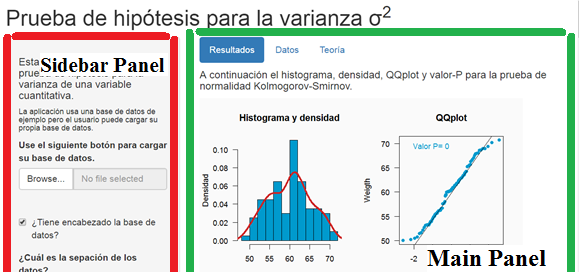
\includegraphics[scale=0.8]{Figura_1}
  \caption{Apariencia del aplicativo web para realizar pruebas de hipótesis para la varianza poblacional}
  \label{figura1}
\end{figure}

En el panel lateral se encuentran los botones (elementos de entrada o inputs) que permitirán al usuario decidir qué hacer con el aplicativo. Las entradas (inputs) que el usuario puede administrar se encuentran en el siguiente orden:

\begin{enumerate}
\item Botón Browse, permite ingresar una base de datos (debe ser un archivo almacenado en su computadora) con las variables de interés o análisis. Los creadores del aplicativo han decidido que cuando el usuario abra el aplicativo, este observé salidas (outputs) o resultados en el panel principal. Esto implica que hay una base de datos cargada de forma predeterminada.

\item Casilla de verificación única (single checkbox), permite “comunicar al aplicativo” si en la base de datos ingresada la primera fila tiene el nombre de las variables, en caso afirmativo dar click sobre la casilla de tal forma que aparezca con relleno (de forma predeterminada la casilla esta con relleno). En caso contrario, dar click en la casilla de tal forma que desaparezca el relleno.

\item Caja de selección (select box) permite al usuario definir el tipo de base de datos que ingresó. Los tipos que admite el aplicativo son:.csv (valores separdos por coma o por punto y coma) y .tsv(valores separados por tabulación). De forma predeterminada esta seleccionada la opción Semicolon.

\item Caja de selección (select box) permite elegir la variable sobre la cual se desea aplicar la prueba de hipótesis de la varianza poblacional. De forma predeterminada esta seleccionada la variable Weigth.

\item Cajón entrada numérica (numeric input) permite definir el valor de la varianza poblacional en la hipótesis nula. De forma predeterminada esta escrito el valor 0.01.

\item Caja de selección (select box) permite definir el tipo de prueba de hipótesis. El usuario puede elegir entre una prueba de hipótesis de dos colas (Diferente) o una cola (hacia la más alta (Mayor) o hacia la más baja (Menor)). De forma predeterminada esta seleccionada la opción Diferente.

\item Deslizador (slider) permite definir el nivel de significancia de la prueba. Tener en cuenta que el nivel de significancia ha sido expresado de tal forma que permita crear un intervalo de confianza. Es decir si el usuario desea un nivel de significancia igual a 0.01, debe posicionar el deslizador en el valor 0.9. De forma predeterminada, el aplicativo inicia con un nivel de significancia igual a 0.05 (el deslizador está posicionado en 0.95).
\end{enumerate}

En la \ref{figura2} se expone los valores de entrada (inputs) seleccionados de forma predeterminada en el panel lateral que el usuario observará cuando abre el aplicativo. Por cuestión de espacio el panel lateral, presentado en la \ref{figura2}, se muestra de forma horizontal, sin embargo al abrir el aplicativo el usuario lo encontrará de forma viertical:

\begin{figure}[h]
  \centering
  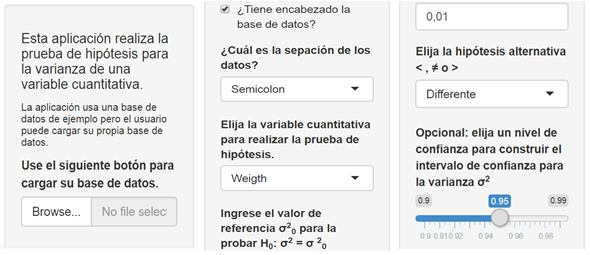
\includegraphics[scale=0.8]{Figura_2}
  \caption{Apariencia del panel lateral}
  \label{figura2}
\end{figure}

En el panel principal el usuario observará las salidas (inputs) producto de las entradas suministradas en el panel lateral. Está estructurado en tres pestañas que el usuario puede elegir con solo dar clic: Resultados, Base de datos y Teoría. De forma predeterminada esta seleccionada la pestaña Resultados.

La pestaña Resultados se encuentra un histograma y un gráfico Q-Q sobre la variable seleccionada que sirven para validar el supuesto de normalidad. Es importante recordar que estos gráficos cambian o se actualizan si el usuario elige otra variable (en el panel lateral elija la variable Heigth y notará el cambio automático). Debajo de los gráficos se presenta una tabla resumen con los estadísticos muestrales: Mínimo, Varianza, Máximo y tamaño muestral. Al final aparece la conclusión de la prueba de hipótesis y un intervalo de confianza de la varianza poblacional.

La base de datos cargada de forma predeterminada o la base de datos que el usuario decida administrar se verá en la pestaña Base de datos. Y la teoría asociada a la prueba de hipótesis que el aplicativo se encarga de aplicar se encuentra en la pestaña Teoría.

La \ref{figura3} muestra la salida (output) en la pestaña Resultados que el usuario observará en el panel principal cuando el usuario abre el aplicativo. Tener en cuenta que esos resultados están en función de las entradas (inputs) seleccionadas en el panel lateral.

\begin{figure}[h]
  \centering
  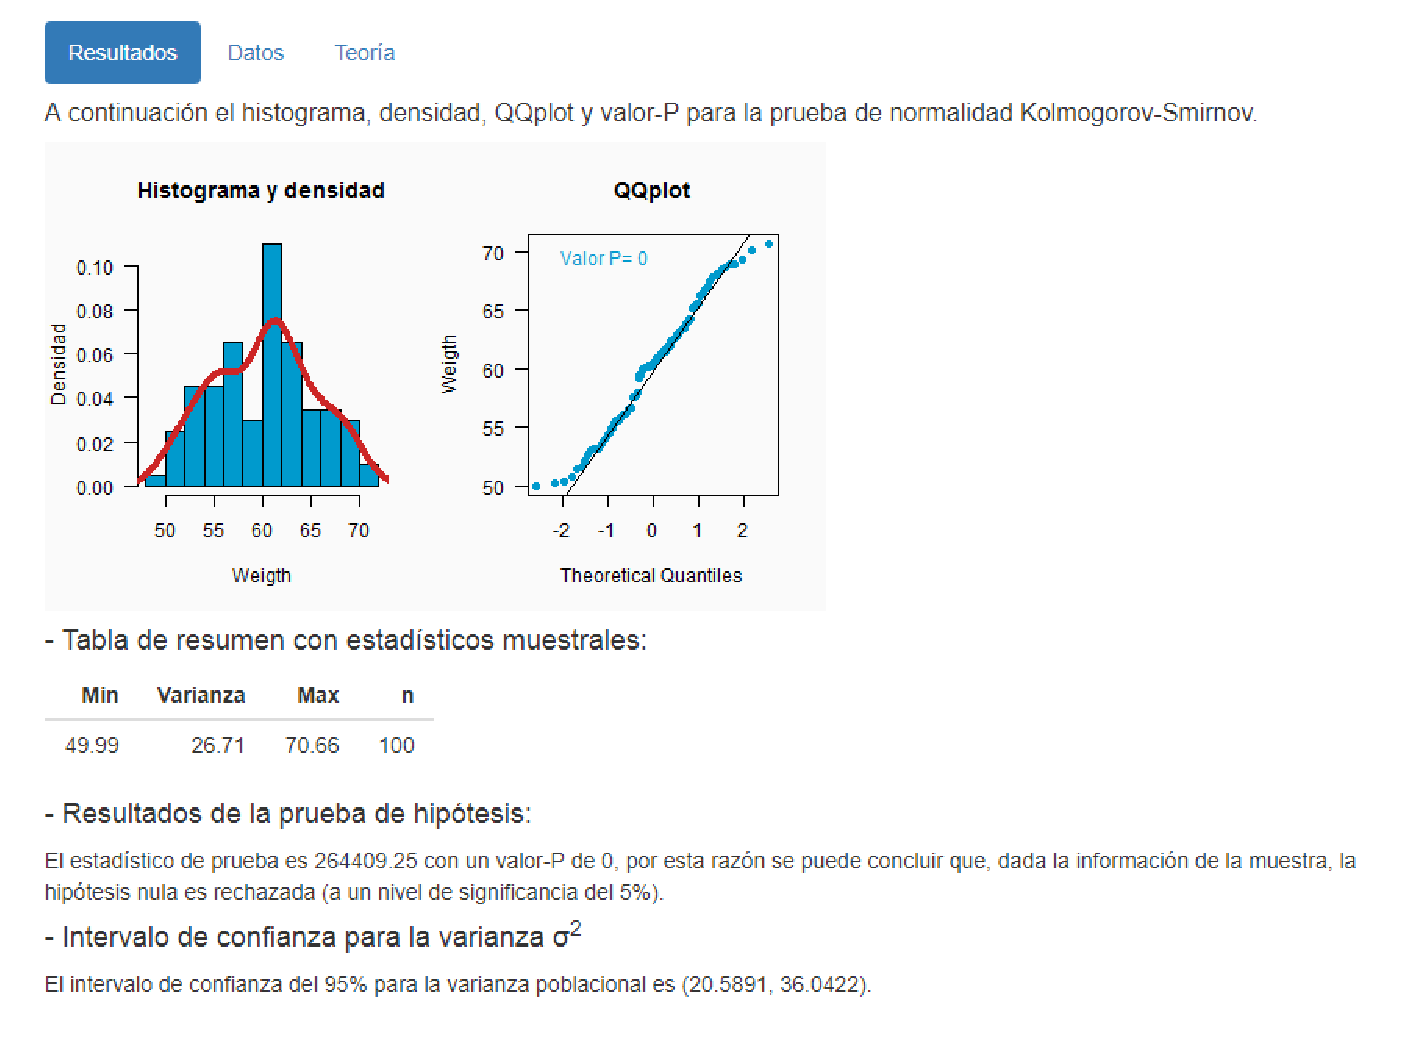
\includegraphics[scale=0.8]{Figura_3}
  \caption{Apariencia del panel principal}
  \label{figura3}
\end{figure}

Se invita al lector a que modifique libremente las entradas (inputs) en el panel lateral o que incluya su propia base de datos para que observé los cambios y cálculos automáticos que realiza el aplicativo.

Tener cuidado con lo siguiente: los cambios o actualizaciones que aparecen en el panel principal dependen de los valores ingresados en el panel lateral, en caso de que no se suministre un valor entonces el aplicativo mostrará un mensaje de error. Esto sólo sucederá si se borra el valor que se encuentra en el cajón de entrada numérica. Se alienta al lentor a que borre dicho valor y note que la tabla con los elementos de la prueba de hipótesis en la pestaña Resultados, y en su lugar surge un mensaje de error: Error: missing value where TRUE/FALSE needed. Para evitarlo no olvide ingresar un valor.


%%%%%%%%%%%%%%%%%%%%%%%%%%%%%%%%%%%%%%%%%%%%%%%%%%%%%%%%%%%%%%%%%%%%%%%%%%%%%%%%%%%%%%%%%%%%%%%%%%%%
\section{Material de apoyo para los docentes}

\textcolor{red}{A cargo de Olga y Freddy.}

%%%%%%%%%%%%%%%%%%%%%%%%%%%%%%%%%%%%%%%%%%%%%%%%%%%%%%%%%%%%%%%%%%%%%%%%%%%%%%%%%%%%%%%%%%%%%%%%%%%%
\section{Conclusiones}

\begin{flushright}
\textbf{Recibido: }\\
\textbf{Aceptado: }
\end{flushright}

% Para la lista de referencias bibliogr?ficas, debe crear un archivo de extension bibtex y usar la siguiente l?nea
\nocite{*}
\references{Bibliografia}


\end{document}